%%%%%%%%%%%%%%%%%%%%%%%%%%%%%%% beamer %%%%%%%%%%%%%%%%%%%%%%%%%%%%%%%%%%%%%%%%%%%%%%%%%
% To run - pdflatex filename.tex
%      acroread filename.pdf
%%%%%%%%%%%%%%%%%%%%%%%%%%%%%%%%%%%%%%%%%%%%%%%%%%%%%%%%%%%%%%%%%%%%%%%%%%%%%%%%%%%%%%%%

\documentclass[compress,oilve]{beamer}
\mode<presentation>

\usetheme[]{CambridgeUS}
% other themes: AnnArbor, Antibes, Bergen, Berkeley, Berlin, Boadilla, boxes, CambridgeUS, Copenhagen, Darmstadt, default, Dresden, Frankfurt, Goettingen,
% Hannover, Ilmenau, JuanLesPins, Luebeck, Madrid, Maloe, Marburg, Montpellier, PaloAlto, Pittsburg, Rochester, Singapore, Szeged, classic

\usecolortheme{beaver}
% color themes: albatross, beaver, beetle, crane, default, dolphin,  fly, lily, orchid, rose, seagull, seahorse, sidebartab, whale, wolverine

\usefonttheme{professionalfonts}
% font themes: default, professionalfonts, serif, structurebold, structureitalicserif, structuresmallcapsserif


\hypersetup{pdfpagemode=FullScreen} % makes your presentation go automatically to full screen

% define your own colors:
\definecolor{Red}{rgb}{1,0,0}
\definecolor{Blue}{rgb}{0,0,1}
\definecolor{Green}{rgb}{0,1,0}
\definecolor{magenta}{rgb}{1,0,.6}
\definecolor{lightblue}{rgb}{0,.5,1}
\definecolor{lightpurple}{rgb}{0.8, 0.6, 0.9}
\definecolor{gold}{rgb}{.6,.5,0}
\definecolor{orange}{rgb}{1,0.4,0}
\definecolor{hotpink}{rgb}{1,0,0.5}
\definecolor{newcolor2}{rgb}{.5,.3,.5}
\definecolor{newcolor}{rgb}{0,.3,1}
\definecolor{newcolor3}{rgb}{1,0,.35}
\definecolor{darkgreen1}{rgb}{0, .35, 0}
\definecolor{darkgreen}{rgb}{0, .6, 0}
\definecolor{darkred}{rgb}{.75,0,0}
\definecolor{skyblue}{HTML}{75bbfd}

\definecolor{olive}{cmyk}{0.64,0,0.95,0.4}
\definecolor{purpleish}{cmyk}{0.75,0.75,0,0}

% can also choose different themes for the "inside" and "outside"

% \usepackage{beamerinnertheme_______}
% inner themes include circles, default, inmargin, rectangles, rounded

% \usepackage{beamerouterthemesmoothbars}
% outer themes include default, infolines, miniframes, shadow, sidebar, smoothbars, smoothtree, split, tree


\useoutertheme[subsection=true, height=40pt]{smoothbars}

% to have the same footer on all slides
%\setbeamertemplate{footline}[text line]{STUFF HERE!}
\setbeamertemplate{footline}[text line]{} % makes the footer EMPTY
% include packages
%

%show the page numbers in footnote
%\addtobeamertemplate{navigation symbols}{}{%
	%	\usebeamerfont{footline}%
	%	\usebeamercolor[fg]{footline}%
	%	\hspace{1em}%
	%	\insertframenumber/\inserttotalframenumber
	%}

\setbeamercolor{footline}{fg=purpleish}
\setbeamerfont{footline}{series=\bfseries}

%add color to curent subsection
\setbeamertemplate{section in head/foot}{\hfill\tikz\node[rectangle, fill=darkred, rounded corners=1pt,inner sep=1pt,] {\textcolor{white}{\insertsectionhead}};}
\setbeamertemplate{section in head/foot shaded}{\textcolor{darkred}{\hfill\insertsectionhead}}

% Remove bullet of subsections
\setbeamertemplate{headline}
{%
	\begin{beamercolorbox}{section in head/foot}
		\insertsectionnavigationhorizontal{\textwidth}{}{}
	\end{beamercolorbox}%
}


% modify headlline, specially headline size
\setbeamertemplate{headline}{%
	\leavevmode%
	\hbox{%
		\begin{beamercolorbox}[wd=\paperwidth,ht=3.5ex,dp=1.125ex]{palette quaternary}%
			\insertsectionnavigationhorizontal{\paperwidth}{}{\hskip0pt plus1filll}
		\end{beamercolorbox}%
	}
}

\setbeamertemplate{footline}{%
	\leavevmode%
	\hbox{\begin{beamercolorbox}[wd=.5\paperwidth,ht=2.5ex,dp=1.125ex,leftskip=.3cm plus1fill,rightskip=.3cm]{author in head/foot}%
			\usebeamerfont{author in head/foot}\insertshortauthor ~ \insertshortinstitute
		\end{beamercolorbox}%
		\begin{beamercolorbox}[wd=.5\paperwidth,ht=2.5ex,dp=1.125ex,leftskip=.3cm,rightskip=.3cm plus1fil]{title in head/foot}%
			\usebeamerfont{title in head/foot}\insertshorttitle\hfill\insertframenumber\,/\,\inserttotalframenumber
	\end{beamercolorbox}}%
	\vskip0pt%
}


%\setbeamertemplate{navigation symbols}{}

\title{Decision Trees}
\author{ML Instruction Team, Fall 2022}
\institute[]{CE Department \newline  Sharif University of Technology \newline \newline}
\date[\today]{}
%\titlegraphic{\includegraphics[scale=.35]{example-image}}



%Write \usepackage{etex} just after the \documentclass line (it should be the first loaded package).
\usepackage{etex}
\usepackage{subcaption}
\usepackage{multicol}
\usepackage{amsmath}
\usepackage{epsfig}
\usepackage{graphicx}
\usepackage[all,knot]{xy}
\xyoption{arc}
\usepackage{url}
\usepackage{multimedia}
\usepackage{hyperref}
\hypersetup{colorlinks,linkcolor=blue,citecolor=redorange,urlcolor=darkred}
\usepackage{multirow}
\usepackage[font={scriptsize}]{caption}
\usepackage{pgf}
\usepackage{fontspec}
%\setsansfont[Scale=MatchLowercase, BoldFont = * Bold, ItalicFont = * Italic]{Caladea}

%\usepackage{enumitem,xcolor}
%\newcommand{\labelitemi}{$\blacksquare$}
%\newcommand{\labelitemii}{$\diamond$}
%\newcommand{\labelitemiii}{$\square$}
%\newcommand{\labelitemiv}{$\ast$}
%\setbeamercolor*{item}{fg=red}


\usefonttheme{professionalfonts} 
\setbeamertemplate{itemize item}{\color{skyblue}$\blacksquare$}
\setbeamertemplate{itemize subitem}{\color{hotpink}$\blacktriangleright$}
\setbeamertemplate{itemize subsubitem}{\color{orange}$\bullet$}


\usepackage{anyfontsize}
\usepackage{t1enc}
\usepackage{tikz}
\usetikzlibrary{calc,trees,positioning,arrows,chains,shapes.geometric,decorations.pathreplacing,decorations.pathmorphing,shapes,matrix,shapes.symbols}



\newtheorem{proposition}[theorem]{Proposition}
\newtheorem{remark}[theorem]{Remark}
\newtheorem{assumption}[theorem]{Assumption}

\usepackage{xcolor}
\newcommand{\tc}[2]{
	\textcolor{#1}{\hspace{-2pt}#2\hspace{-2pt}}
}

%\usepackage{fontspec, unicode-math}
%\setmainfont[Scale=0.9]{Nimbus Roman No9 L}
%\setmonofont[Scale=0.9]{Monaco}
\setsansfont[Scale=1]{Times New Roman}

\newcommand{\vect}[1]{\boldsymbol{#1}}

\definecolor{strings}{rgb}{.624,.251,.259}
\definecolor{keywords}{rgb}{.224,.451,.686}
\definecolor{comment}{rgb}{.322,.451,.322}


%\usepackage{smartdiagram}
%\usesmartdiagramlibrary{additions}
%%%%%%%%%%%%%%%%%%%%%%%%%%%%%%%%%%%%%%%%%%%%%%%%%%%%%%%%%%%%%%%%%%%%%%%%%%%%%%%%%%%%%%%%%%%%
%%%%%%%%%%%%%%%%%%%%%%%%%%%%%% Title Page Info %%%%%%%%%%%%%%%%%%%%%%%%%%%%%%%%%%%%%%%%%%%
%%%%%%%%%%%%%%%%%%%%%%%%%%%%%%%%%%%%%%%%%%%%%%%%%%%%%%%%%%%%%%%%%%%%%%%%%%%%%%%%%%%%%%%%%%


%%%%%%%%%%%%%%%%%%%%%%%%%%%%%%%%%%%%%%%%%%%%%%%%%%%%%%%%%%%%%%%%%%%%%%%%%%%%%%%%%%%%%%%%%%
%%%%%%%%%%%%%%%%%%%%%%%%%%%%%% Begin Your Document %%%%%%%%%%%%%%%%%%%%%%%%%%%%%%%%%%%%%%%
%%%%%%%%%%%%%%%%%%%%%%%%%%%%%%%%%%%%%%%%%%%%%%%%%%%%%%%%%%%%%%%%%%%%%%%%%%%%%%%%%%%%%%%%%%
\begin{document}
	
%%%%%%%%%%%%%%%%%%%%%%%%%%%%%%%%%%%%%%%%%%%%%%%%%%%%%%%%%%%%%%%%%%%%%%%%%%%%%%%%%%%%%%%%%%
\fontsize{9}{9}
\begin{frame}[noframenumbering, plain]
	\titlepage
\end{frame}

%%%%%%%%%%%%%%%%%%%%%%%%%%%%%%%%%%%%%%%%%%%%%%%%%%%%%%%%%%%%%%%%%%%%%%%%%%%%%%%%%%%%%%%%%%
\section{Introduction}
%%%%%%%%%%%%%%%%%%%%%%%%%%%%%%%%%%%%%%%%%%%%%%%%%%%%%%%%%%%%%%%%%%%%%%%%######
\frame{\frametitle{Decision Tree}
	
	\begin{itemize}
		\item \tc{keywords}{Decision Tree} algorithms can be considered as an iterative, top-down construction
		method for either classifier or regressor.
		
		\item 
		\medskip
		Considering only binary (or Boolean) features, at each node, there are $2^m$ potential splits to be evaluated given that the dataset has $m$ features.
		
		\begin{figure}
			\centering
			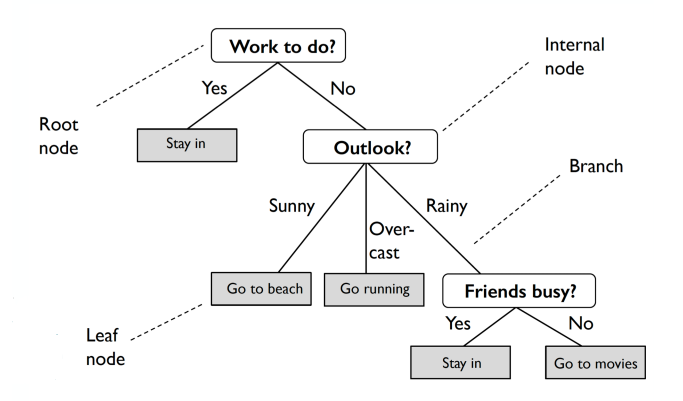
\includegraphics[width=8cm, height=4.5cm]{Figs/task.PNG}
			\caption{Decision Tree, \href{https://tinyurl.com/2hwn5d2z}{Source}}
			\label{fig:decision tree}
		\end{figure}
		
	\end{itemize}


}
%%%%%%%%%%%%%%%%%%%%%%%%%%%%%%%%%%%%%%%%%%%%%%%%%%%%%%%%%%%%%%%%%%%%%%%%%%%
\frame{\frametitle{Terminology}
	
	\begin{itemize}
		\item \tc{keywords}{Root Node}: No incoming edge, zero, or more outgoing edges.
		
		\medskip
		\item \tc{keywords}{Internal Node}: One incoming edge, two (or more) outgoing edges.
		
		\medskip
		\item \tc{keywords}{Leaf Node}: Each leaf node is assigned a class label if nodes are pure; otherwise, the class label is determined by majority vote.
		
		\medskip
		\item \tc{keywords}{Parent \& Child Node}: If a node is split, we refer to that given node as the parent node, and the resulting nodes are called child nodes.
		
		\begin{figure}
			\centering
			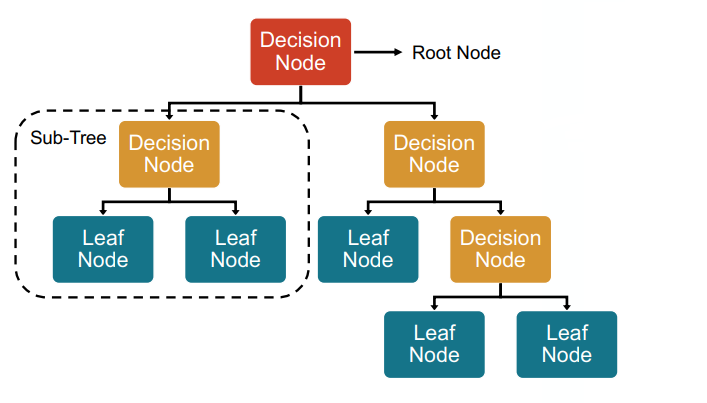
\includegraphics[width=6cm, height=3.5cm]{Figs/terminology.png}
			\caption{Terminology, \href{https://tinyurl.com/2n2w6jws}{Source}}
			\label{fig:terminology}
		\end{figure}
		
	\end{itemize}


}
%%%%%%%%%%%%%%%%%%%%%%%%%%%%%%%%%%%%%%%%%%%%%%%%%%%%%%%%%%%%%%%%%%%%%%%%
\section{Algorithm}
%%%%%%%%%%%%%%%%%%%%%%%%%%%%%%%%%%%%%%%%%%%%%%%%%%%%%%%%%%%%%%%%%%%%%%%%
\frame{\frametitle{Information Gain}
	
	\begin{itemize}
		\item \tc{keywords}{Entropy}: Let $X$ be a random variable over a discrete space $\Omega$ with probability mass function $\mathbb{P}$. Then the (Shannon) entropy of $X$ is:
		\begin{equation*}
			H(X)=\mathbb{E}_X[\log(\frac{1}{\mathbb{P}(X)})]=\sum_{x \in X} \mathbb{P}(x) \log \frac{1}{\mathbb{P}(x)}=-\sum_{x \in X} \mathbb{P}(x) \log \mathbb{P}(x)
		\end{equation*}
	
	\item Upper Bound for $H(x)$:
	\begin{itemize}
		\item Jensen Inequality:
		\begin{equation*}
			H(X)=\mathbb{E}\left(\log \frac{1}{\mathbb{P}_X(X)}\right)
			\leq \log \mathbb{E}\left(\frac{1}{\mathbb{P}_X(X)}\right)
			=\log|X|
		\end{equation*}
	
	\item Using Lagrange multipliers with the constraint $\sum_x p(x)=1$:
	
	\begin{equation*}
		H(x) \leq-\sum_x \frac{1}{|X|} \log(\frac{1}{|X|})=\log (|X|)
	\end{equation*}
	
	
	
	\end{itemize}

	\medskip
	\item \tc{keywords}{Gini Impurity}: Let $X$ be a random variable over a discrete space $\Omega$ with probability mass function $\mathbb{P}$. Then the gini coefficient of $X$ is:
	\begin{equation*}
		G(X)=\sum_{x \in X}\mathbb{P}(x)(1-\mathbb{P}(x))=1-\sum_{x \in X}\mathbb{P}(x)^2
	\end{equation*}
	
	\end{itemize}
	
}
%%%%%%%%%%%%%%%%%%%%%%%%%%%%%%%%%%%%%%%%%%%%%%%%%%%%%%%%%%%%%%%%%%%%%%%%%%%
\frame{\frametitle{Information Gain}
	\begin{figure}
		\centering
		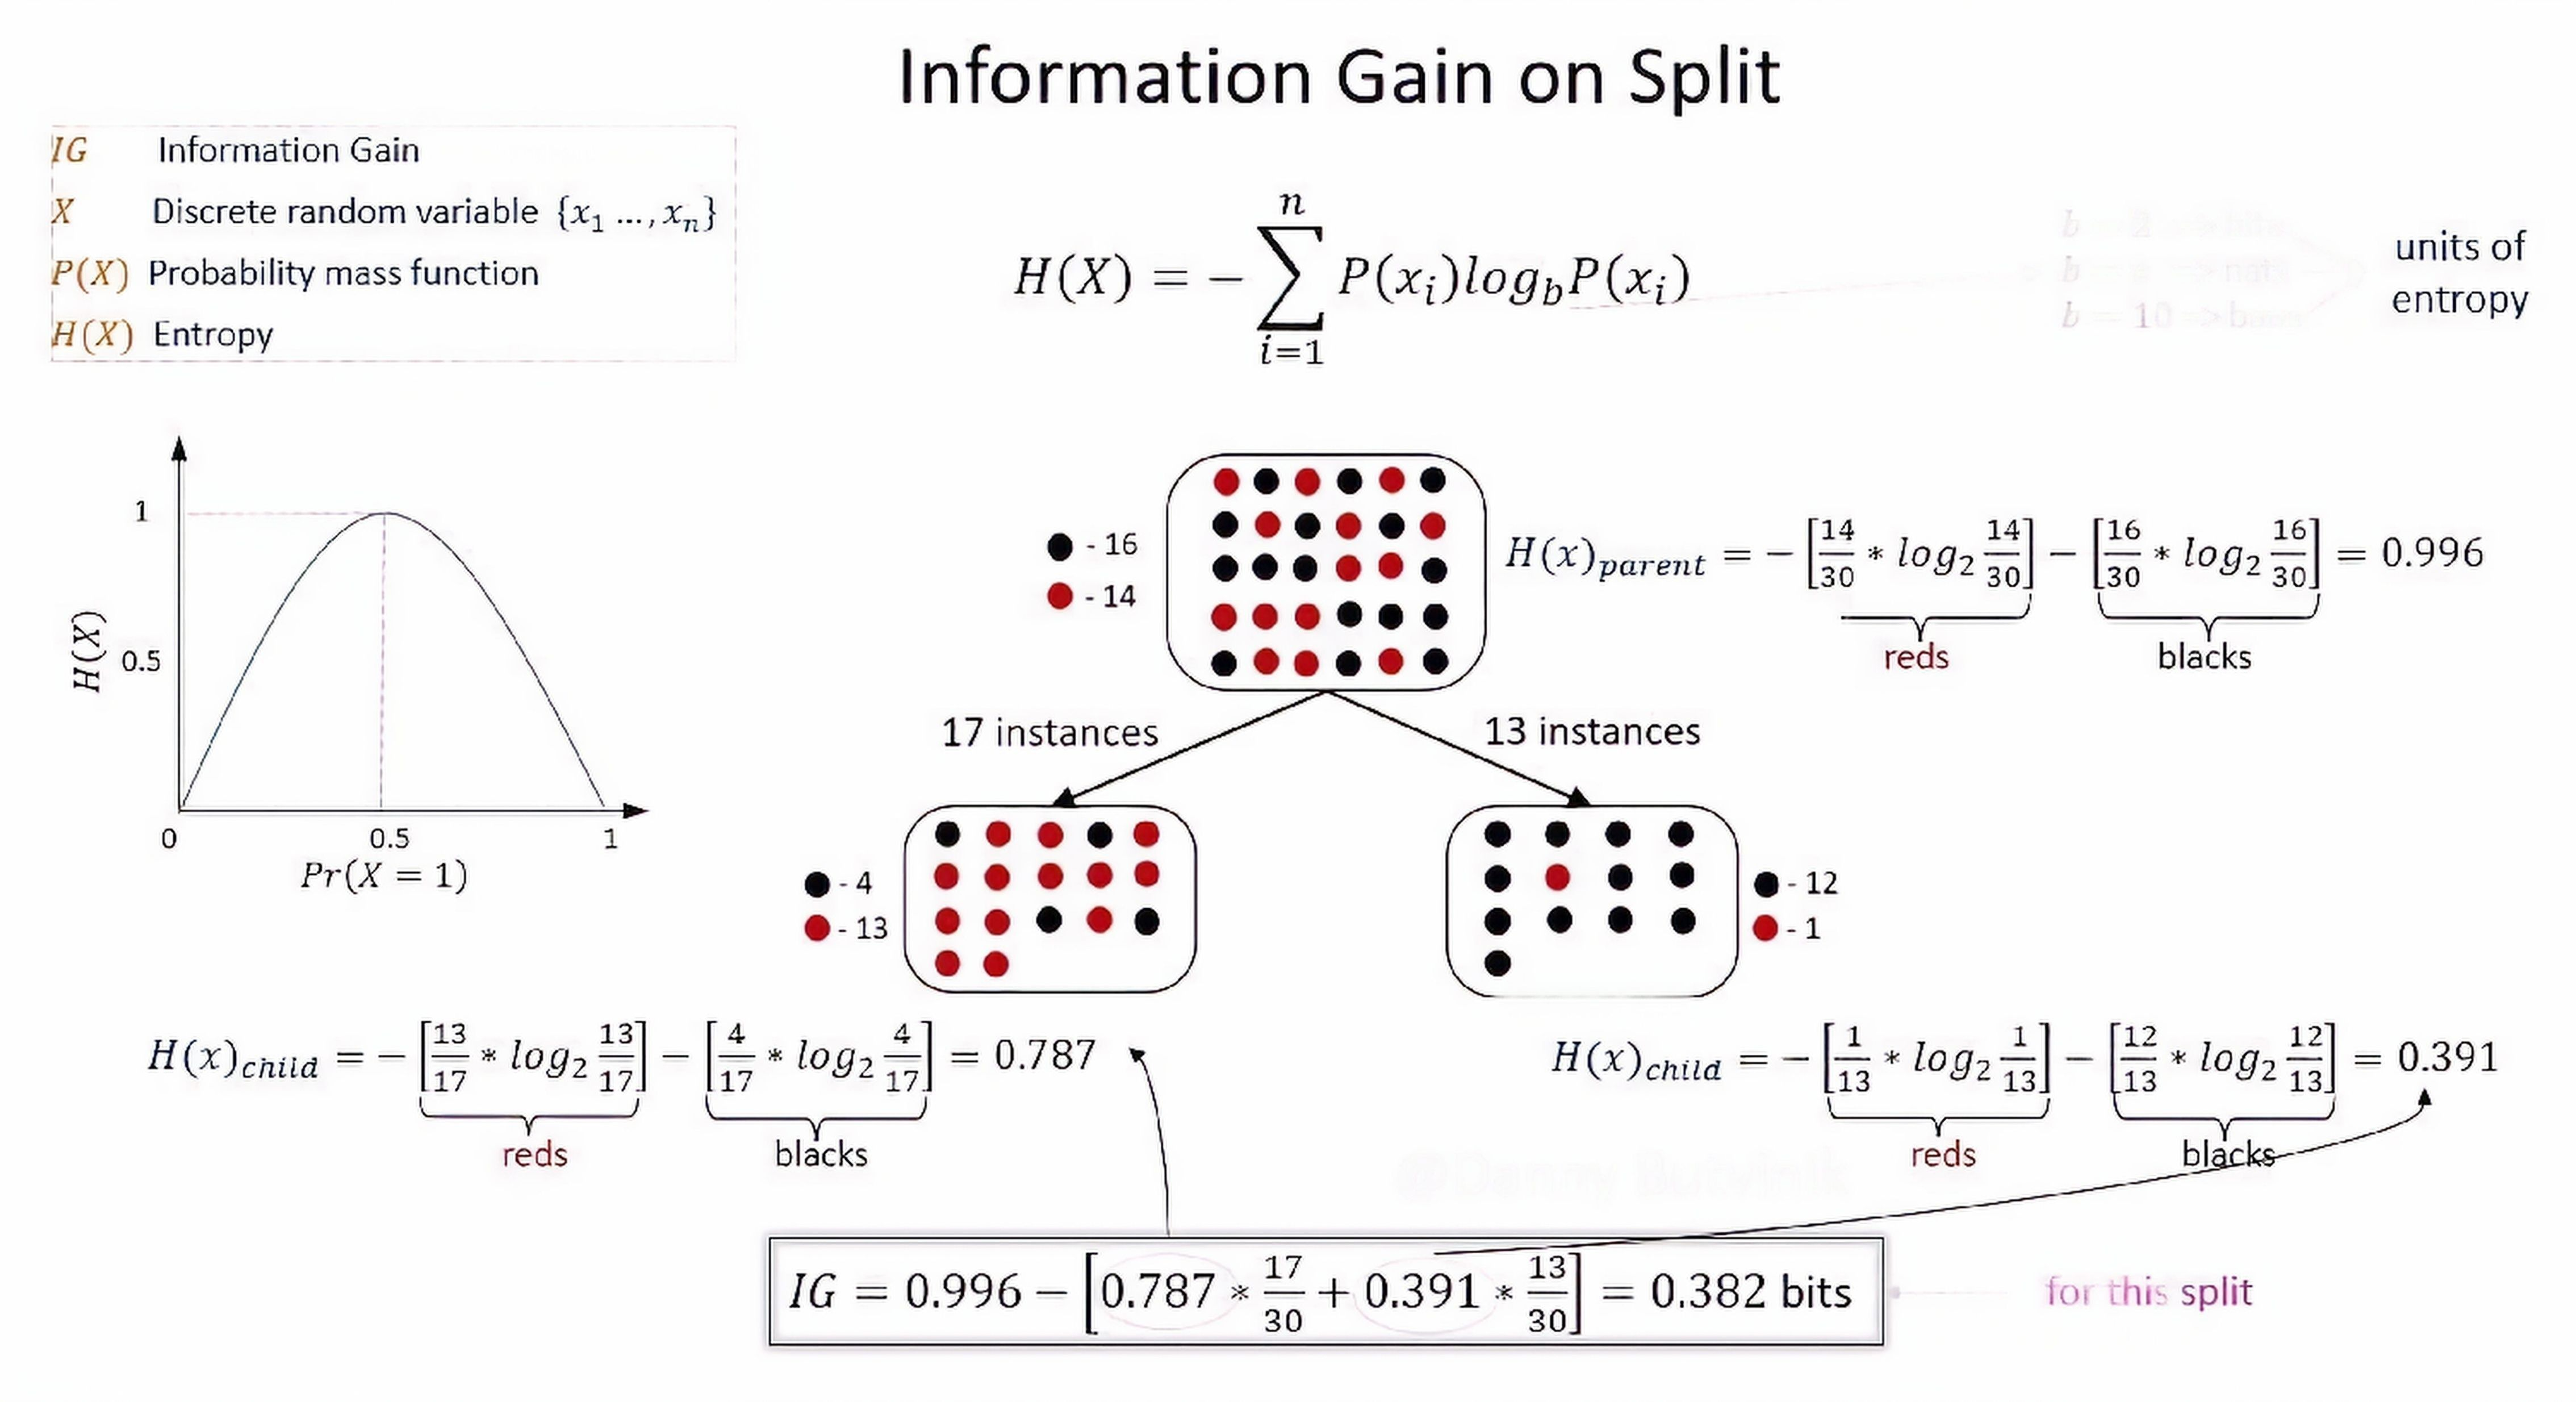
\includegraphics[width=12cm, height=6cm]{Figs/IG.jpeg}
		\caption{Information Gain, \href{https://tinyurl.com/2n2w6jws}{Source}}
		\label{fig:information gain}
	\end{figure}

}

%%%%%%%%%%%%%%%%%%%%%%%%%%%%%%%%%%%%%%%%%%%%%%%%%%%%%%%%%%%%%%%%%%%%%%%%%%%
\frame{\frametitle{CART Algorithm}
	\vspace{-1.5cm}
\begin{itemize}
	\item The algorithm first splits the training set in \tc{keywords}{two subsets} using a \tc{keywords}{single feature} $k$ and a \tc{keywords}{threshold} $t_k$. 
	
	\medskip
	\item How does it choose $k$ and $t_k$?\\
	It searches for the
	pair $(k, t_k)$ producing the \tc{keywords}{purest subsets}, which are weighted by their size.
	
	\medskip
	\item Once it has successfully split the training set in two, it splits the \tc{keywords}{subsets} using the same logic, then the \tc{keywords}{sub-subsets} and so on, recursively.
	
	\medskip 
	\item \tc{keywords}{CART} algorithm is a greedy algorithm: it greedily searches for an optimum split at the top level, then repeats the
	process at each level.
	
	\medskip
	\item It does not check whether or not the split will lead to the lowest possible impurity several levels down.
\end{itemize}
}
%%%%%%%%%%%%%%%%%%%%%%%%%%%%%%%%%%%%%%%%%%%%%%%%%%%%%%%%%%%%%%%%%%%%%%%
\frame{\frametitle{Decision Trees in Practice}
	\begin{figure}
		\centering
		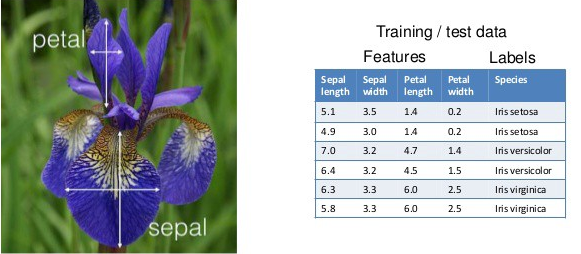
\includegraphics[width=9cm, height=5cm]{Figs/iris_info.png}
		\caption{Iris Dataset, \href{https://tinyurl.com/2ebkm4bs}{Source}}
		\label{fig:iris-dataset}
	\end{figure}
	
}

%%%%%%%%%%%%%%%%%%%%%%%%%%%%%%%%%%%%%%%%%%%%%%%%%%%%%%%%%%%%%%%%%%%%%%%%
\frame{\frametitle{Decision Trees in Practice}
	\begin{figure}
		\centering
		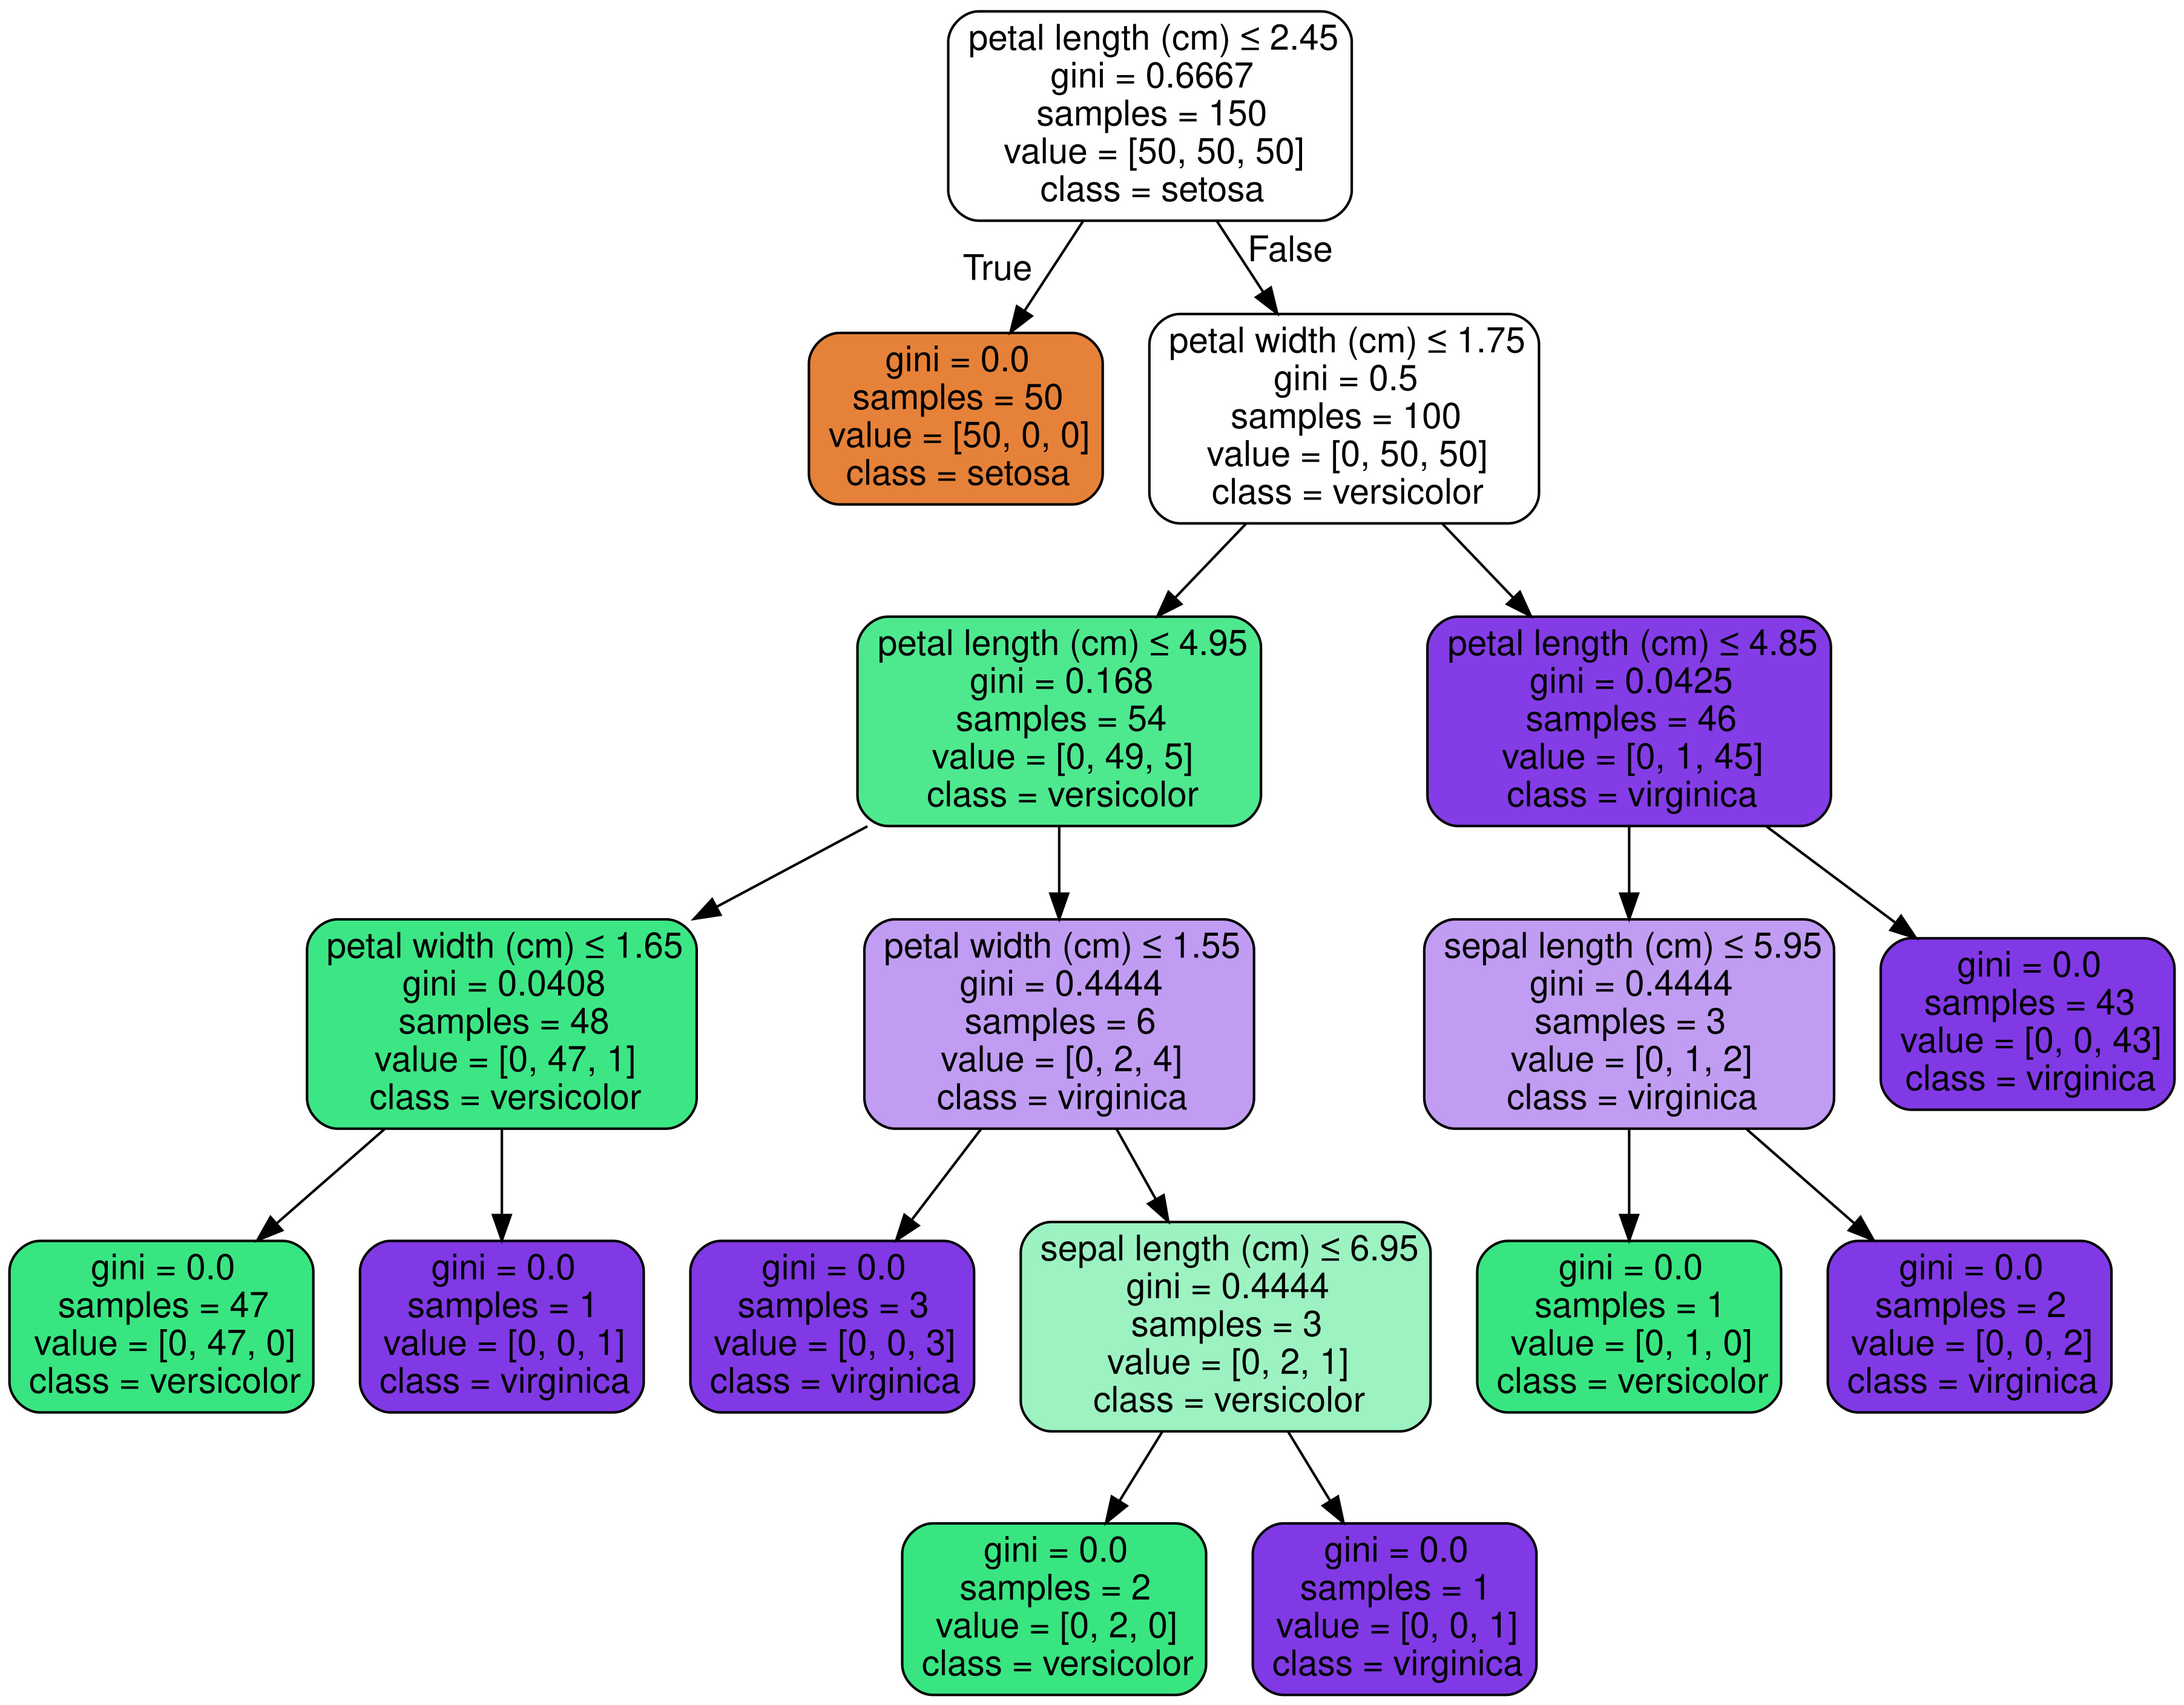
\includegraphics[width=10cm, height=6.5cm]{Figs/iris.jpg}
		\caption{Decision Trees on Iris Dataset, \href{https://tinyurl.com/2zhuxgn6}{Source}}
		\label{fig:decision trees-sklearn}
	\end{figure}

}

%%%%%%%%%%%%%%%%%%%%%%%%%%%%%%%%%%%%%%%%%%%%%%%%%%%%%%%%%%%%%%%%%%%%%%%%%%%
\frame{\frametitle{Misclassifications Error}
	\vspace{-1.5cm}
	\begin{itemize}
		\item \tc{keywords}{Misclassification} error seems to
		be another reasonable choice, where:
		
		\begin{equation*}
			E R R(\mathcal{D})=\frac{1}{n} \sum_{i=1}^n L(\hat{y}^{[i]}, y^{[i]})
		\end{equation*}
		with the 0-1 Loss,
		\begin{equation*}
			L(\hat{y}, y)=\{\begin{array}{l}
				0 \text { if } \hat{y}=y, \\
				1 \text{ if }  \hat{y}\neq y
			\end{array}
		\end{equation*}
	
		\item
		\medskip
		This, in case of the training set, is equal to
		\begin{equation*}
			E R R(p)=1-\max _i(p(i \mid x_j))
		\end{equation*}
		
		for a given node if we use majority voting at this node.
		
		\medskip
		\item Can we apply this measure as the criteria for splitting?
	\end{itemize}


}

%%%%%%%%%%%%%%%%%%%%%%%%%%%%%%%%%%%%%%%%%%%%%%%%%%%%%%%%%%%%%%%%%%%%%%%%%%
\frame{\frametitle{Misclassifications Error}
	\begin{figure}[htbp!]
		\subfloat[][Misclassification Error, \href{https://tinyurl.com/2gswcjmd}{Source}]
		{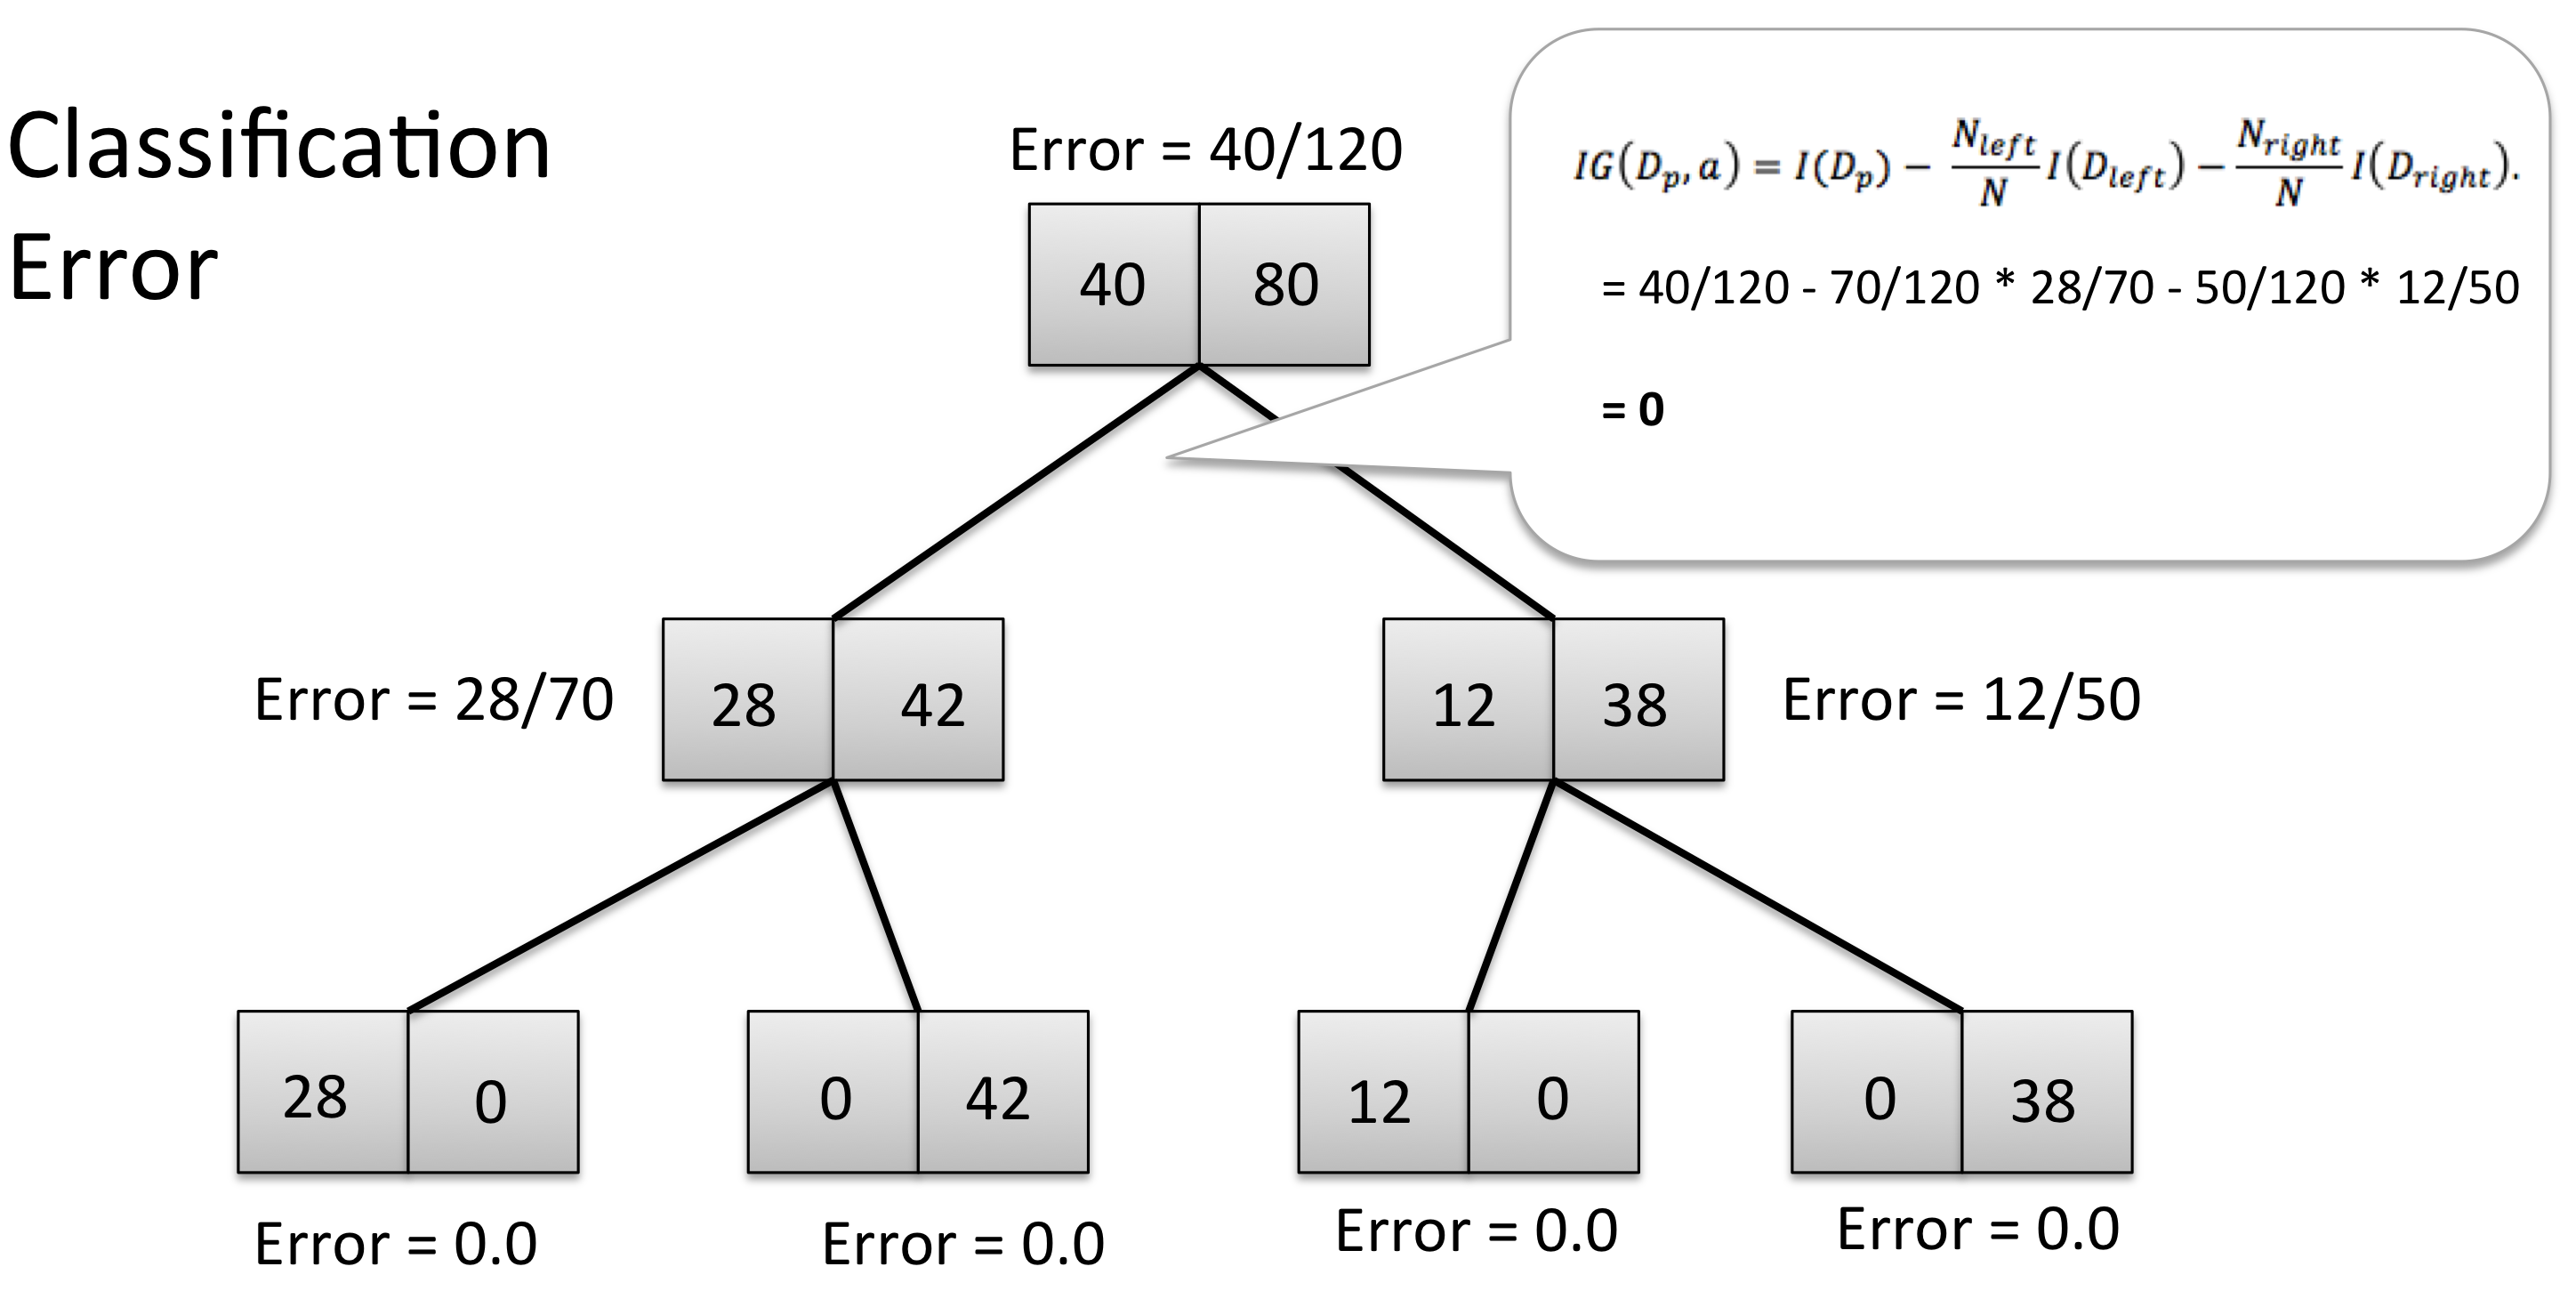
\includegraphics[width=8cm, height=3.25cm]{Figs/misclassification_criterion.png}
			\label{fig:subfigure1}}
		
		\subfloat[][Entropy, \href{https://tinyurl.com/2hjbcvpr}{Source}]
		{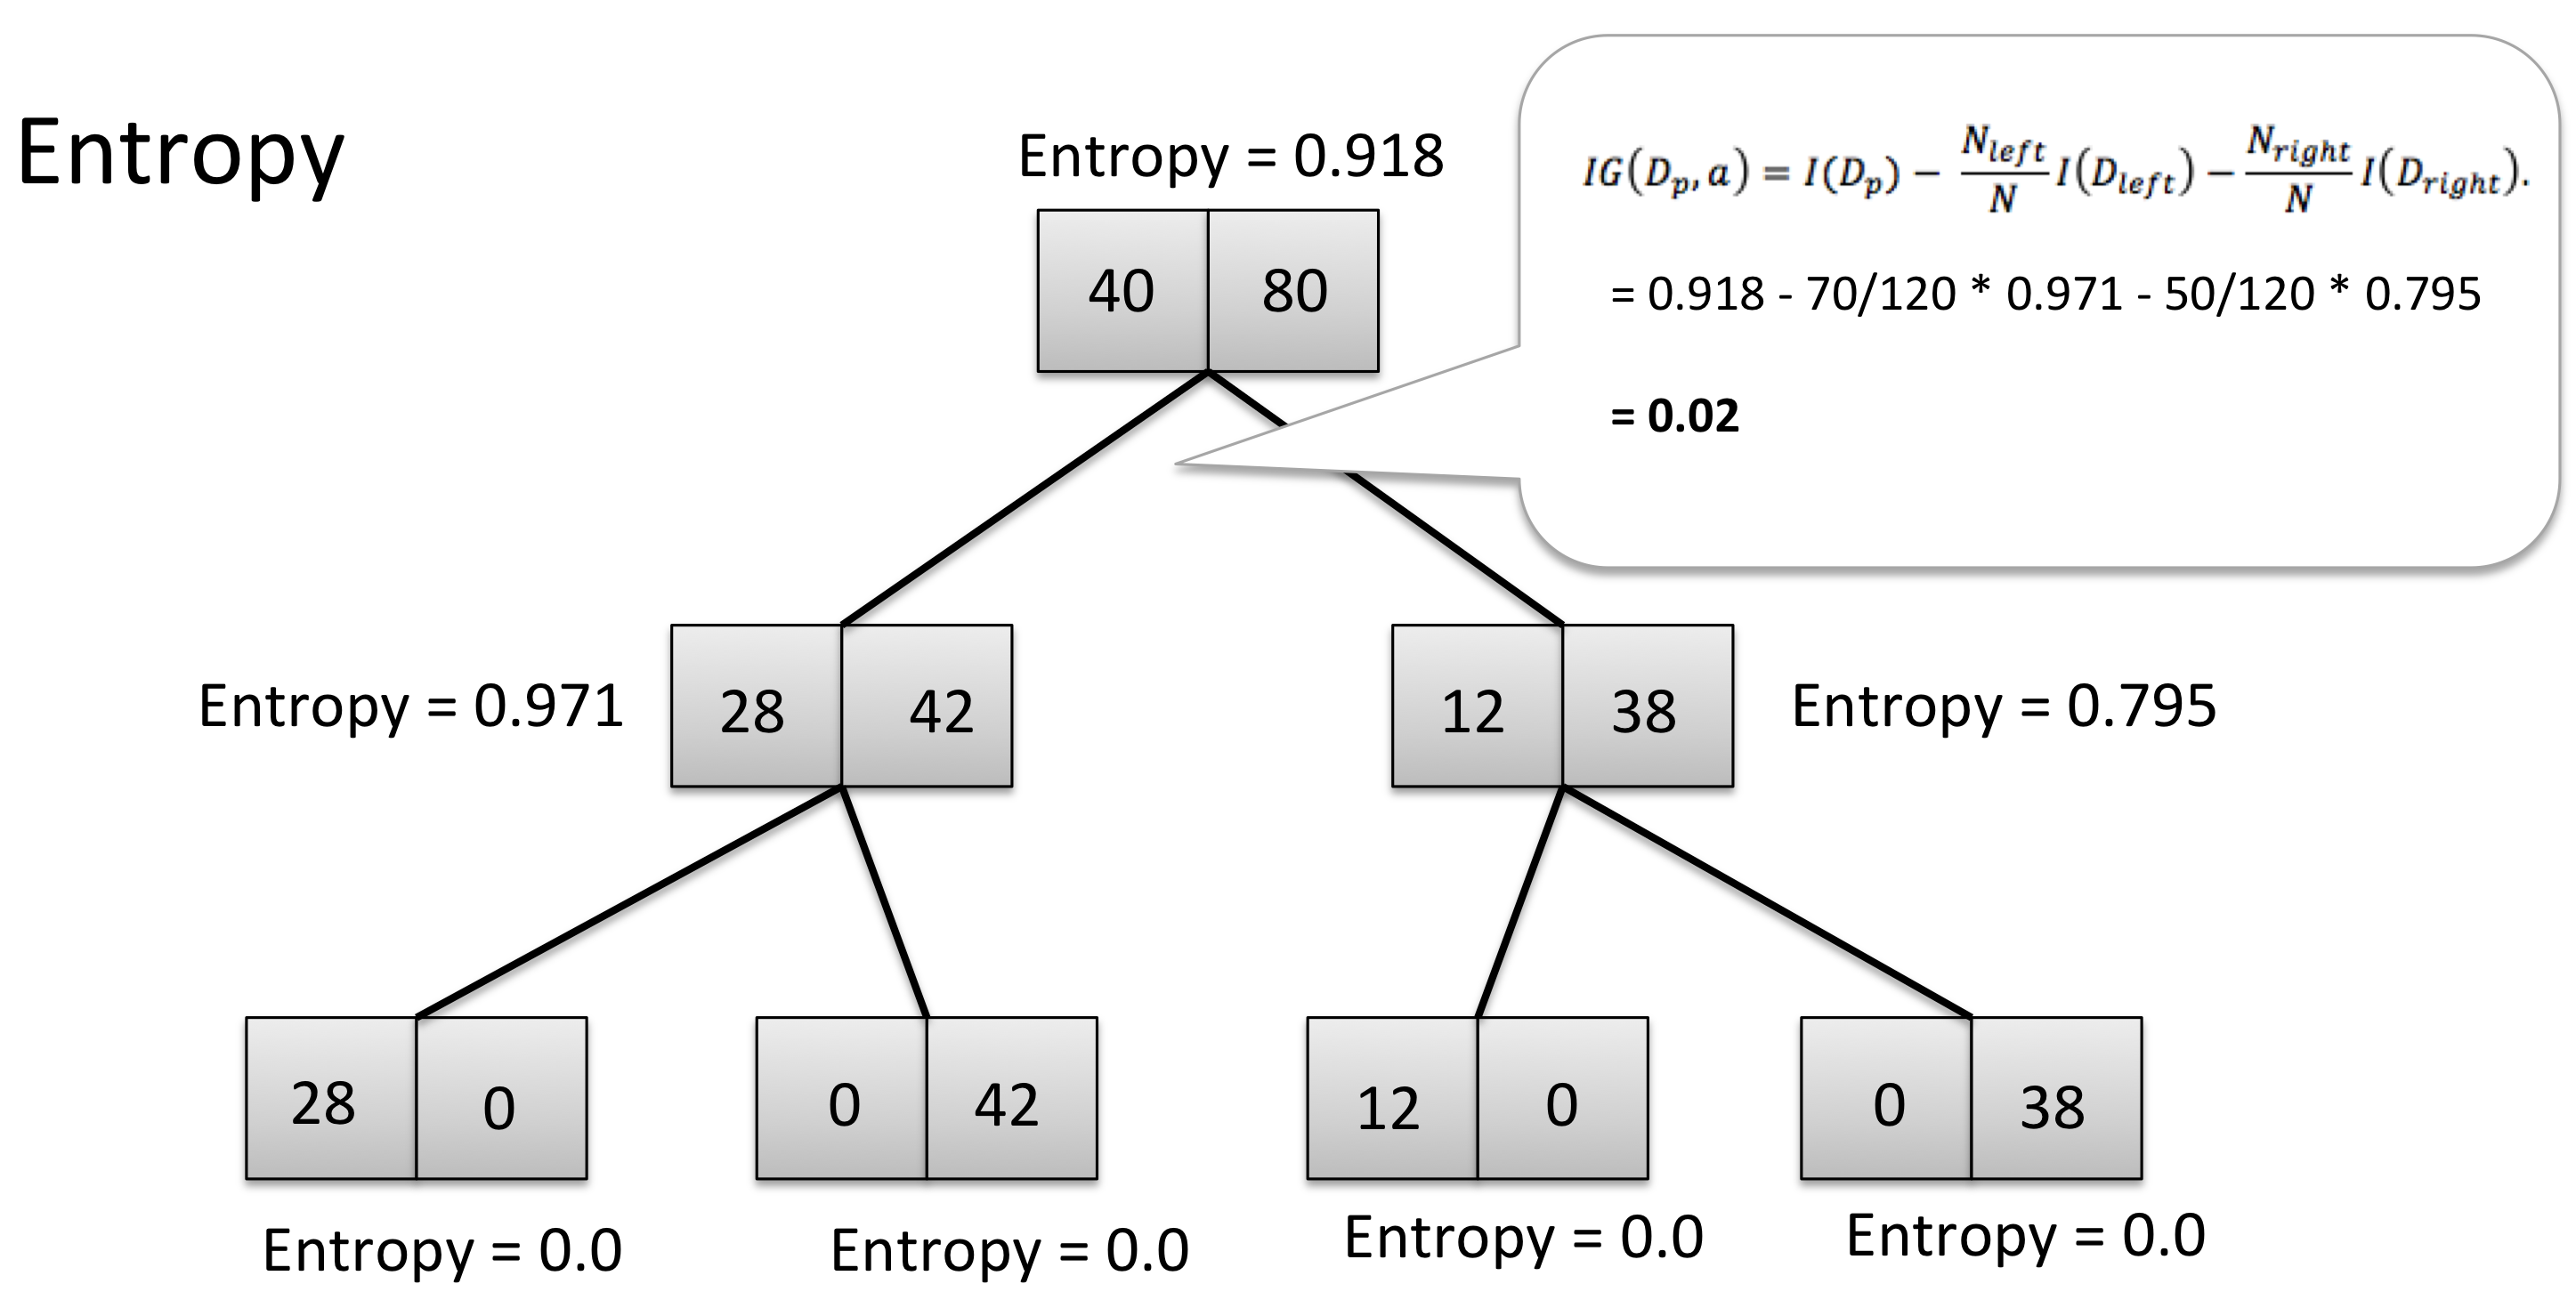
\includegraphics[width=8cm, height=3.5cm]{Figs/entropy_criterion.PNG}
			\label{fig:subfigure2}}
		\label{fig:globalfigure2}
		
	\end{figure}
}
%%%%%%%%%%%%%%%%%%%%%%%%%%%%%%%%%%%%%%%%%%%%%%%%%%%%%%%%%%%%%%%%%%%%%%%%%%
\frame{\frametitle{Positiveness of Information Gain}
		\begin{figure}
			\centering
			\vspace{-1cm}
			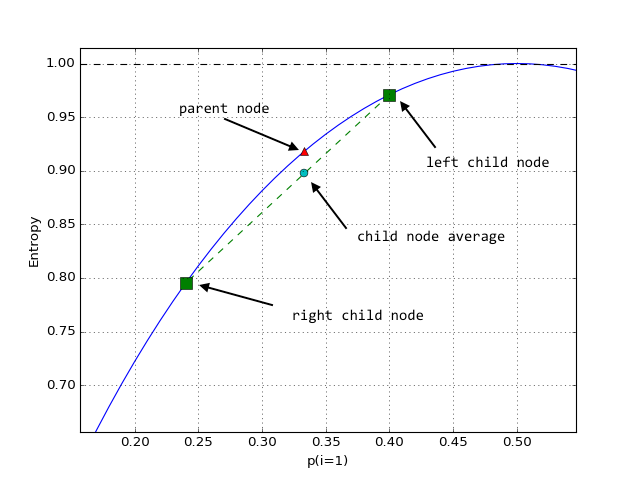
\includegraphics[width=10cm, height=7cm]{Figs/IG-Concave.png}
			\caption{Concavity of Entropy, \href{https://tinyurl.com/2zcn3bbx}{Source}}
			\label{fig:positiveness of information gain}
		\end{figure}
		
	}

%%%%%%%%%%%%%%%%%%%%%%%%%%%%%%%%%%%%%%%%%%%%%%%%%%%%%%%%%%%%%%%%%%%%%%%%%%
\section{Pros and Cons}

%%%%%%%%%%%%%%%%%%%%%%%%%%%%%%%%%%%%%%%%%%%%%%%%%%%%%%%%%%%%%%%%%%%%%%%%%%
\frame{\frametitle{Overfitting}
\begin{itemize}
	\item Decision Trees make very few assumptions about the training data!
	
	\medskip
	\item If left unconstrained, their structure will adapt itself to the training data, fitting it very closely, and most likely overfitting it!
	
	\medskip
	\item To avoid overfitting the training data, you need to restrict the Decision Tree’s freedom during training.
	
	\item Which parameters can be restricted?
	
	\medskip
	\begin{itemize}
		\item \tc{keywords}{Max Tree Depth}: Maximum depth of the tree.
		
		\medskip
		\item \tc{keywords}{Max Leaf Nodes}: Maximum number of leaf nodes.
		
		\medskip
		\item \tc{keywords}{Min Sample Leaf}: Minimum number of samples a leaf node must have.
		
		\medskip
		\item \tc{keywords}{Min Sample Split}: Minimum number of samples a node must have before it can be split.
		
		\medskip
		\item \tc{keywords}{Max Features}: Maximum number of features that are evaluated for splitting at each node)
	\end{itemize}
\end{itemize}
}
%%%%%%%%%%%%%%%%%%%%%%%%%%%%%%%%%%%%%%%%%%%%%%%%%%%%%%%%%%%%%%%%%%%%%%%%%%%
\frame{\frametitle{Other Algorithms}
\begin{itemize}
	\item ID3: Iterative Dichotomizer 3
	\begin{itemize}
		\item It can only be used for discrete features, and cannot handle numeric features!
		
		\item It supports multi-category splits.
		
		\item  It does not apply any pruning, and is prone to overfitting.
		
		\item It results in short and wide trees (compared to CART).
		
		\item It maximizes information gain/minimizes entropy.
		
	\end{itemize}

	\bigskip
	\item C4.5:
	\begin{itemize}
		\item It supports  Continuous and discrete features (continuous feature splitting is very expensive because must consider all possible ranges).
		
		\item It can handles missing attributes (ignores them in information gain computation)
		
		\item It performs post-pruning 
		
	\end{itemize}
	
\end{itemize}
}
%%%%%%%%%%%%%%%%%%%%%%%%%%%%%%%%%%%%%%%%%%%%%%%%%%%%%%%%%%%%%%%%%%%%%%%%%%
\frame{\frametitle{Decision Trees for Regression}
\begin{itemize}
	\item It is the same as classification with a few subtle modifications:
	
	\begin{itemize}
		\item  The main difference is that instead of predicting a class in each node, it predicts a value.
		
		\medskip
		\item  The prediction for each node is simply the average target value of the all training instances associated to this leaf node.
		
		\medskip
		\item Instead of trying to split the training set in a way that minimizes impurity, CART algorithm now tries to split the
		training set in a way that minimizes the \tc{keywords}{MSE}.
		
		\medskip
		\item The MSE at a given node is also often referred to as \tc{keywords}{intra-node variance}, and the splitting criterion is thus called \tc{keywords}{variance reduction}.
		
		\medskip
		\item Likewise to classification tasks, decision trees are prone to overfitting when dealing with regression tasks.
	\end{itemize}
\end{itemize}

}


%%%%%%%%%%%%%%%%%%%%%%%%%%%%%%%%%%%%%%%%%%%%%%%%%%%%%%%%%%%%%%%%%%%%%%%%%%
\frame{\frametitle{Positiveness of Information Gain}
	\begin{figure}
		\centering
		\vspace{0cm}
		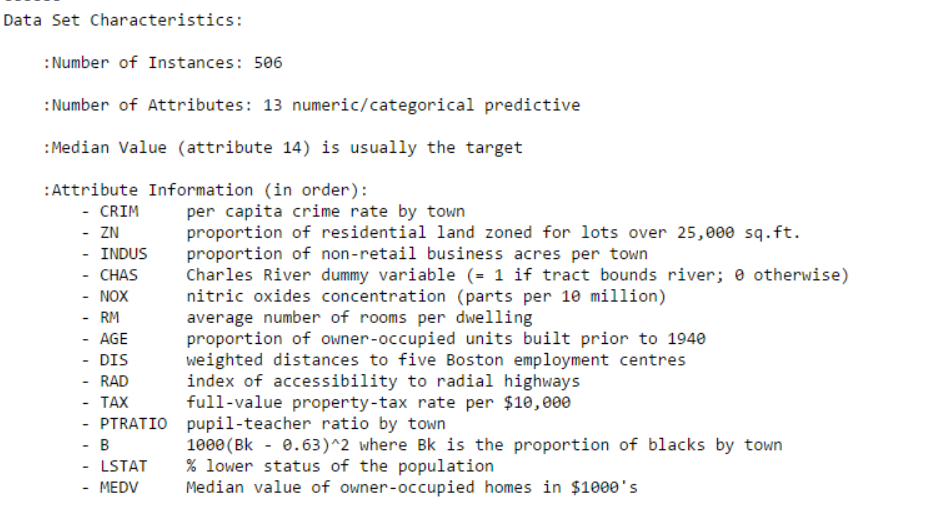
\includegraphics[width=10cm, height=6cm]{Figs/Boston-House-Price-Dataset.png}
		\caption{Boston Dataset, \href{https://tinyurl.com/2ersy9gf}{Source}
		}
		\label{fig:bosoton dataset}
	\end{figure}
	
}
%%
%%%%%%%%%%%%%%%%%%%%%%%%%%%%%%%%%%%%%%%%%%%%%%%%%%%%%%%%%%%%%%%%%%%%%%%%%%%
\frame{\frametitle{Decision Trees for Regression}
	\begin{figure}
		\centering
		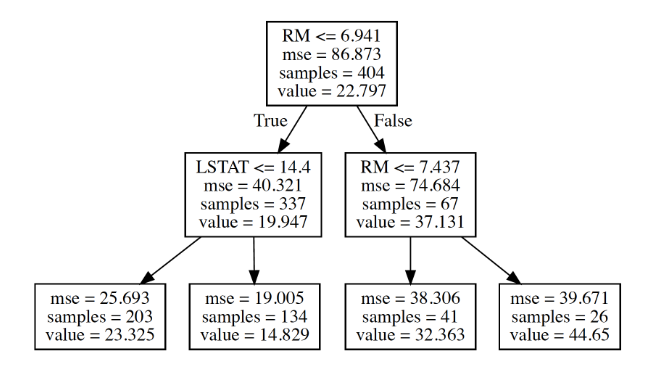
\includegraphics[width=10cm, height=6cm]{Figs/decision_trees_MSE.png}
		\caption{Concavity of Entropy, \href{https://tinyurl.com/2zcn3bbx}{Source}}
		\label{fig:information gain-concave}
	\end{figure}
	
}
%%%%%%%%%%%%%%%%%%%%%%%%%%%%%%%%%%%%%%%%%%%%%%%%%%%%%%%%%%%%%%%%%%%%%%%%%%%
\frametitle{Final Notes}
\centering
\vspace{50 pt}
\textbf{Thank You!}
\vspace{50pt}

\textbf{Any Question?}
%%%%%%%%%%%%%%%%%%%%%%%%%%%%%%%%%%%%%%%%%%
\end{document}